\chapter{Verwandte Arbeiten}

Der Bereich der Konsistenzprüfung zwischen strukturbasierten und verhaltensbasierten Modellen ist seit Jahren gut erforscht.
Insbesondere gibt es ein großes Spektrum an Methoden zum Vergleichen von verschiedenen UML-Modellen.
Viele dieser Methoden untersuchen die Konsistenz zwischen UML-Klassendiagrammen und UML-Verhaltensmodellen wie UML-Zustands- oder UML-Aktivitätsdiagramme.
Da sich die Konzepte dieser UML-Modelle mit denen von BROS und BPMN ähneln, lassen sich diese Methoden auch auf BPMN- und BROS-Modelle anwenden.
Dafür wird zunächst ein Klassifikationsschema für Verfahren zur Konsistenzprüfung vorgestellt.
Anhand dieses Schemas werden anschließend relevante Arbeiten erläutert und verglichen.

\section{Klassifikationsschema für Verfahren zur Konsistenzprüfung}

Da es bereits etliche Arbeiten im Gebiet der Konsistenzprüfung von UML-Modellen gibt, wurde bereits eine Zusammenstallung der bestehenden Methoden von  \cite{Usman2008} und \cite{Lucas2009} durchgeführt.
Um die unterschiedlichen Methoden besser klassifizieren zu können nutzen beide Arbeiten ein ähnliches Klassifikationsschema:

\begin{itemize}
    \item \textbf{Nature (\cite{Usman2008}):} Es beschreibt den Fokus der vergleichbaren Modelltypen. Dabei wird zwischen strukturbasierten und verhaltensbasierten Modellen unterschieden. Strukturbasierte Modelle beschreiben den Aufbau eines Systems. Dazu zählen unter anderem UML-Klassen-, UML-Komponentendiagramm und BROS-Modelle. Zu den verhaltensbasierten Modellen gehören beispielsweise UML-Zustands-, UML-Aktivitätsdiagramme und BPMN-Modelle. Diese Modelle verdeutlichen den die Abläufe und Zustände innerhalb eines Systems. Mögliche Werte sind strukturbasiert, verhaltensbasiert und beides.
    \item \textbf{Diagrams (\cite{Usman2008}):} Es beschreibt welche konkreten Modelle von der Methode unterstützt werden. Die Arbeiten von \cite{Usman2008} und \cite{Lucas2009} beziehen sich dabei ausschließlich auf UML Diagramme. Mögliche Werte sind die Modellnamen.
    \item \textbf{Consistency Type (\cite{Usman2008}):} Es beschreibt welche Arten der Konsistenz von der Methode überprüft werden. Dabei wird hauptsächlich unterschieden zwischen \emph{Inter-Modell (vertikale) Konsistenz} (Konsistenz bei verschiedenen Abstraktionsstufen und gleichem Modelltyp), \emph{Intra-Modell (horizontale) Konsistenz} (Konsistenz bei gleicher Abstraktionsstufe und verschienden Modelltypen)und \emph{Evolutionskonsistenz} (Konsistenz der eines Modelles über verschiedende Entwicklungsstufen). Zusätzlich spezifiziert \cite{Usman2008} noch die \emph{semantische-} und die \emph{syntaktische Konsistenz}. Diese Beziehen sich auf die Konsistenz eines Modelles zu seinem Metamodell. Dies wird für die nachfolgende Arbeit als Vorraussetzung angesehen und nicht näher betrachtet.
    \item \textbf{Consistency Strategy (\cite{Usman2008}):} Es beschreibt die benutzte Validierungsstrategie. Es werden drei verschiedene Strategien genannt und zwar \emph{Analysis} (Auf einem Algorithmus basierend), \emph{Monitoring} (Auf einem Regelsatz basierend) und \emph{Construction} (Auf der Generierung des zu vergleichenden Modelles basierend).
    \item \textbf{Intermediate Representation (\cite{Usman2008}):} Es beschreibt ob die Methode eine temporäre Zwischendarstellung benötigt oder nicht. Mögliche Werte sind ja und nein. 
    \item \textbf{Case Study (\cite{Usman2008}):} Es beschreibt ob die Methode an einem Beispiel evaluiert wurde. Mögliche Werte sind ja und nein. 
    \item \textbf{Automatable (\cite{Usman2008}):} Es beschreibt ob die Methode manuell oder automatisiert von einem Programm durchgeführt werden kann. Mögliche Werte sind gut (H), mittel (M) und schlecht (L).
    \item \textbf{Tool Support (\cite{Usman2008}):} Es beschreibt ob die Methode von einem Tool unterstützt wird oder ein eigenes Tool entwickelt wurde. Mögliche Werte sind ja und nein.
    \item \textbf{Model Extensibility:} Es beschreibt wie gut die Methode um weitere Modelle für den Konsistenzvergleich erweiterbar ist. Mögliche Werte sind gut (H), mittel (M) und schlecht (L).
    \item \textbf{Rule Extensibility:} Es beschreibt wie gut die Methode um weitere Konsistenzregeln erweiterbar ist. Mögliche Werte sind gut (H), mittel (M) und schlecht (L).
\end{itemize}

Dieses Schema ist direkt auf die Konsistenzprüfung von BPMN- und BROS-Modelle anwendbar.
Wichtig für die weitere Arbeit sind Methoden deren \emph{Nature} beide Modelltypen unterstützt und deren \emph{Consistency Type} auf der \emph{Intra-Modell (horizontale) Konsistenz} beruht.
Den Aspekt der Erweiterbarkeit wird von \cite{Lucas2009} genannt.
Da ein Hauptziel dieser Arbeit die Erweiterbarkeit ist wird dieser Aspekt nocheinmal untergliederd.

\section{Aktuelle Verfahren zur Konsistenzprüfung}

\textbf{Transformation zu \emph{CSP-OZ}:}
\cite{Rasch2003} transformiert Klassen- und Zustandsdiagramme nach \emph{CSP-OZ} (Communicating Sequential Processes - Object-Z) als Zwischendarstellung.
\emph{CSP} ist eine Prozessalgebra für die Beschreibung der Zusammenarbeit verschiedener Systeme. 
\emph{OZ} ist eine objektorientierte Erweiterung der Z-Notation. Diese wird zur formalen Beschreibung von Systemen genutzt.
Anhand eines Regelsatzes wird die Konsistenz der Zwischendarstellungen geprüft.
\cite{Kim2004} nutzt ein ähnliches Verfahren, spezialisiert sich dabei aber nur auf Zustandsdiagramme.

\textbf{Transformation zu \emph{Pertinetze}:}
\cite{Shinkawa2006} zeigt das verhaltensbasierte UML-Modelle in \emph{CPN} (Coloured Petri Net) überführt werden können.
Mittels mehrerer Beispiele werden verschiedene Transformationsstrategien gezeigt.
Die formale \emph{Inter-Modell (vertikale) Konsistenz} der CPNs wird nur theoretisch behandelt.
Bernardi et al. (\cite{Usman2008}, 13) nutzt GSPN (Generalized stochastic Petri nets) anstelle von CPN. \textit{TODO: Vorteil von GSPN?}

\textbf{Anwendung von \emph{Description logic}:}
\cite{Mens2005} nutzt \emph{Description logic} für die formale Konsistenzprüfung.
Dabei werden beide Modelltypen und alle Validierungsstrategien unterstützt.
Für die \emph{Evolutionskonsistenz} wird eine Erweiterung des UML-Metamodells erstellt.
Zusätzlich führt \cite{Mens2005} eien Fallstudie durch und entwickelt eine Toolunterstützung.
Ein ähnlicher Ansatz wird von \cite{Simmonds2004} genutzt.
Noch weiter geht Satoh et al. (\cite{Usman2008}, 15) indem UML-Klassendiagramme direkt in Logikprogramme übersetzt und ausgeführt werden.

\textbf{Transformation in ein gemeinsames Modell:}
\cite{Egyed2001} entwickelt die ViewIntegra Methode für die  \emph{Inter-Modell (vertikale)} und \emph{Intra-Modell (horizontale) Konsistenz}.
Der Fokus der ViewIntegra Methode liegt in der Skalierbarkeit und Effizienz der Überprüfung bei großen Modellen.
Um dies zu erreichen wird eine iterative Umwandlung von verwandten UML-Modellen beschrieben.
Dieses iterative Vorgehen reduziert den Entwicklungsaufwand erheblich da nun nur noch ein Bruchteil aller benötigten Transformationsalgorithmen entwickelt werden muss.
Dies vereinfacht auch die Erweiterbarkeit um neue Modellarten.
Die konstruierten Modelle können anschließend direkt mittels \emph{Inter-Modell (vertikale) Konsistenz} überprüft werden.
Einige der beschrieben Transformationsalgorithmen sind bereits implementiert wurden.
Aufgrund der Umwandlung wird auch die \emph{Intra-Modell (horizontale) Konsistenz} unterstützt.

\textbf{Nutzung von UML-Constraints wie \emph{OCL}:}
\cite{Egyed2006} prüft die Konsistenz zwischen UML-Klassen-, Sequenz- und Zustandsdiagrammen mittels OCL-Regeln.
Neben einer Fallstudie wurde auch ein Tool entwickelt um das Verfahren zu testen.
Aufgrund von Einschränkungen von OCL, wie das Fehlen des transitiven Abschlusses, ist die Erweiterbarkeit dieses Ansatzes eingeschränkt.
\cite{Briand2003} verwendet ebenfalls OCL-Regeln, konzentriert sich dabei aber auf die \emph{Evolutionskonsistenz}.

\section{Vergleich der bestehenden Verfahren}

\begin{figure}
    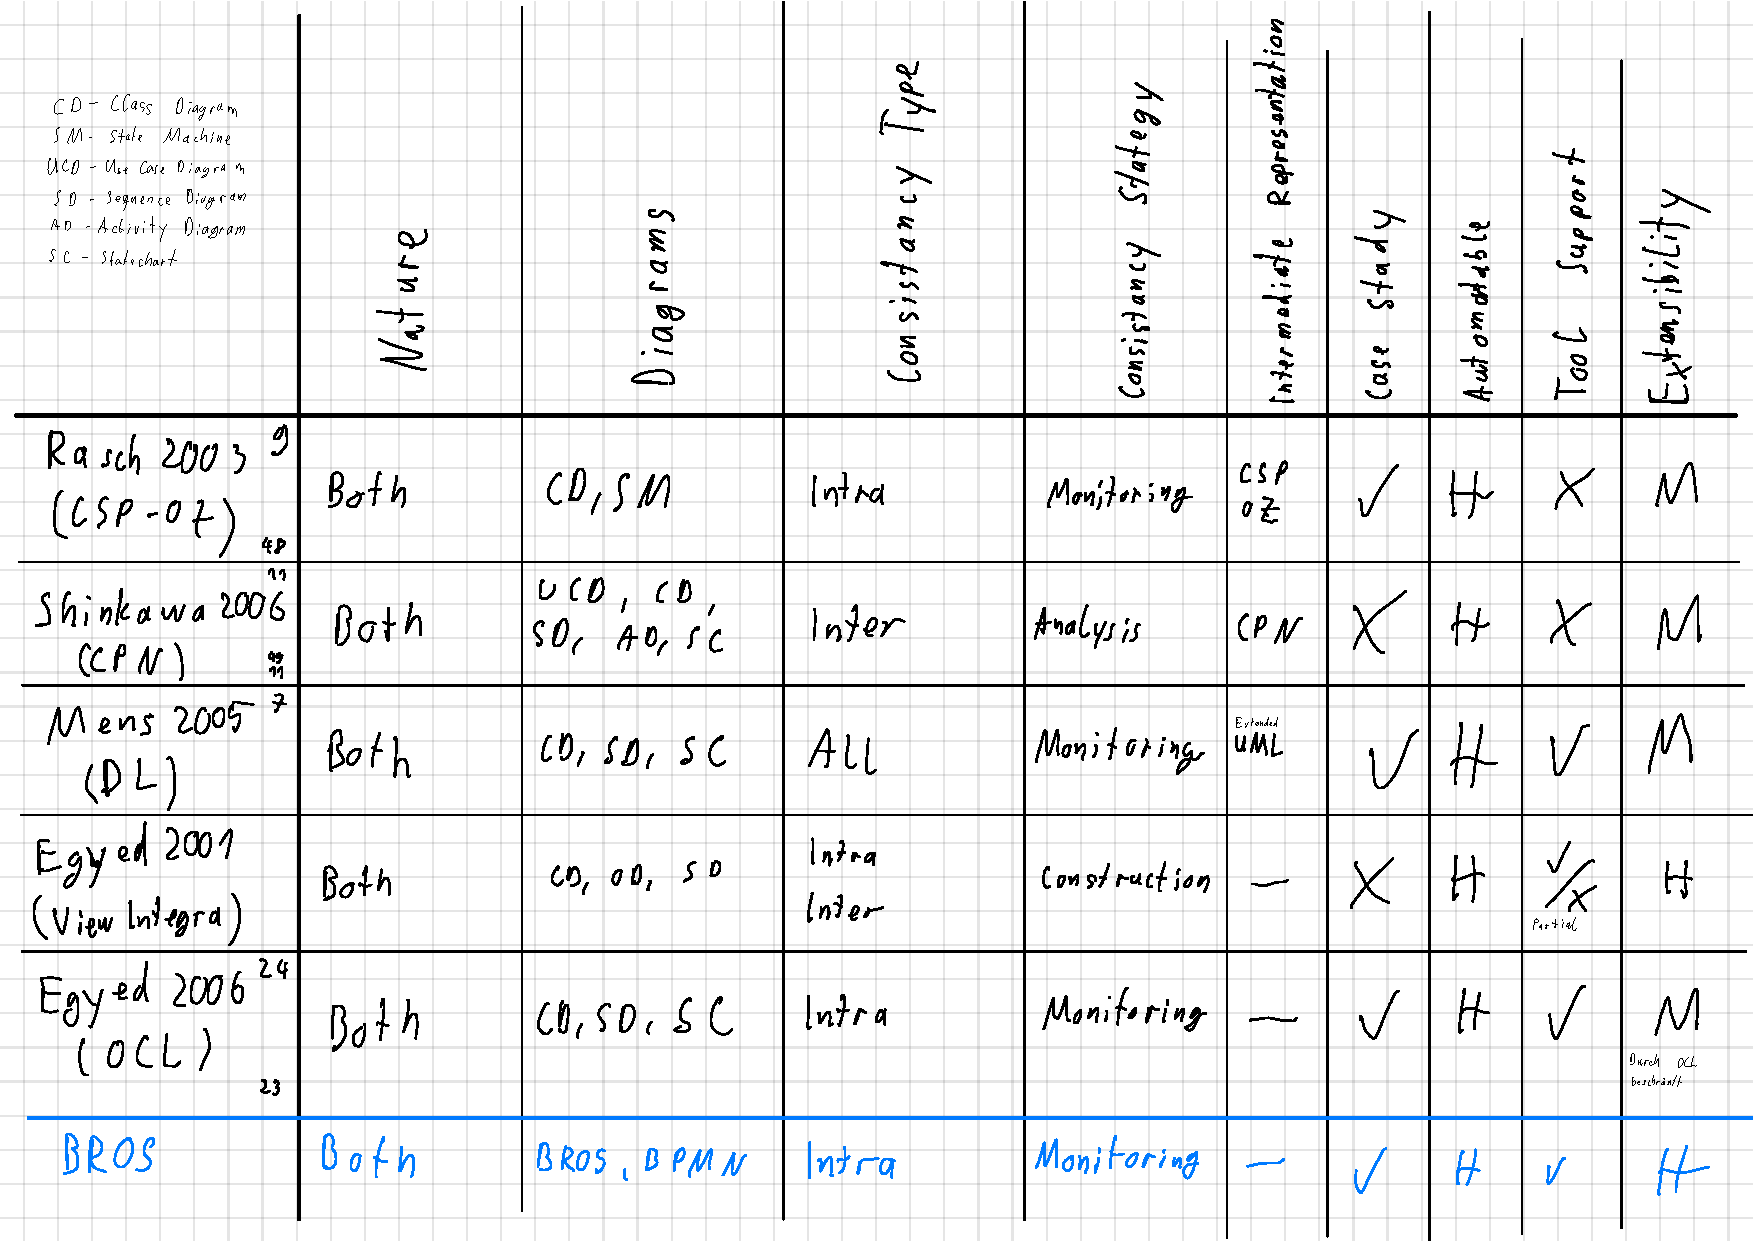
\includegraphics[width=\textwidth,keepaspectratio]{../images/Klassifikationsschema.pdf}%
    \caption{Vergleich der bestehenden Verfahren}%
    \label{fig:klassifikationsschema}
\end{figure}

Die fünf beschriebenen Verfahren lassen sich in zwei Kategorien teilen.
Zum einen die die eine Zwischendarstellung benötigen und die die keine Zwischendarstellung nutzen.
\cite{Rasch2003}, \cite{Shinkawa2006} und \cite{Mens2005} beschreiben Verfahren die zunächst eine Zwischendarstellung aufbauen und anschließend die Konsistenz der Zwischendarstellung überprüfen.
Andererseits könne die Verfahren von \cite{Egyed2001} und \cite{Egyed2006} direkt auf den Modellen arbeiten.
Der große Vorteil ist die leichte Erweiterbarkeit um neue Modellarten.
Es muss nur eine neue Konvertierungsmethode des Modelles zur Zwischendarstellung entwickelt werden.
Anschließend können die gleichen Algorithmen zur Konsistenzprüfung wie bei den bestehenden Modellen verwendet werden.
Allerdings ist dies auch eine Beschränkung der Erweiterbarkeit.
Eine allgemeine Form der Zwischendarstellung hat zumeist den Nachteil des Informationsverlustes.
Dadurch lassen sich nur schwer neue Regeln für die Konsistenz Zwischendarstellung hinzufügen.
Es kann auch sein das eine Modellart nicht kompatibel zu der Zwischendarstellung ist.
Dann ist eine Erweiterung nicht möglich.
Dagegen haben die Verfahren ohne Zwischendarstellung weniger Beschränkungen der Erweiterbarkeit.
Hier ist das größte Hindernis der Aufwand eine neue Modellart hinzuzufügen.
Im schlechtesten Fall müssen beim Hinzufügen einer neuen Modellart N neue Konvertierungsmethoden entwickelt werden.
\cite{Egyed2001} umgeht dieses Problem mittels einer iterativen Transformation.

Die am meisten benutzte Methode zur Konsistenzprüfung ist das \emph{Monitoring} (vgl. \cite{Usman2008}).
Das \emph{Monitoring} basiert auf der Konsistenzprüfung mittels eines Regelsatzes. 
Verfahren die \emph{Monitoring} nutzen, haben eine gute Erweiterbarkeit im bezug auf neue Konsistenzregeln.
Dazu zählen die Verfahren von \cite{Rasch2003}, \cite{Mens2005} und \cite{Egyed2006}.
\emph{Monitoring} bietet allerdings keine formale Verifikation, sondern nur eine Überprüfung vergleichbar mit Unittests.
Dies wird von dem Verfahren der \emph{Analysis} gelöst.
Mittels formaler Verifikation kann die Konsistenz bewiesen werden.
Allerdings sind solcher Verfahren nicht sehr flexibel.
Bei \cite{Shinkawa2006} kann beispielsweise nur die \emph{Inter-Modell (vertikale) Konsistenz} verifiziert werden.
Die dritte Methode, die \emph{Construction}, beschreibt Verfahren deren Hauptaufgabe die Konstruktion anderer Modelle ist.
Verfahren die mit einem Transformationsalgorithmus eine Zwischendarstellung konstruieren, zählen nicht dazu.
\cite{Egyed2001} nutzt diese Methode und beschreibt die Transformation zwischen verschiedenen UML-Modellen.
Die Konsistenzprüfung der Modelle erfolgt mittels \emph{Inter-Modell (vertikale) Konsistenz} und ist unabhängig von dem Konstruktionsverfahren.
Da die eigentliche Konsistenzprüfung nicht teil eines Konstruktionsverfahrens ist, kann diese Methode orthogonal zu den anderen beiden Methoden verwendet werden.
